% Created 2019-05-16 Thu 08:15
\documentclass[9pt, b5paper]{article}
\usepackage{fontspec}
\usepackage{graphicx}
\usepackage{xcolor}
\usepackage[slantfont,boldfont]{xeCJK}
\setCJKmainfont[BoldFont = Heiti SC, ItalicFont = STFangsong]{STSong}
\setCJKsansfont{STHeiti}
\setCJKmonofont{STFangsong}
\usepackage{multirow}
\usepackage{multicol}
\usepackage{float}
\usepackage{textcomp}
\usepackage{geometry}
\geometry{left=1.2cm,right=1.2cm,top=1.5cm,bottom=1.0cm}
\usepackage{algorithm}
\usepackage{algorithmic}
\usepackage{latexsym}
\usepackage{natbib}
\usepackage{listings}
\usepackage{minted}
\usepackage[xetex,colorlinks=true,CJKbookmarks=true,linkcolor=blue,urlcolor=blue,menucolor=blue]{hyperref}
\author{deepwaterooo}
\date{\today}
\title{Android NDK 开发笔记}
\hypersetup{
  pdfkeywords={},
  pdfsubject={},
  pdfcreator={Emacs 25.3.1 (Org mode 8.2.7c)}}
\begin{document}

\maketitle
\tableofcontents


\section{Android 之 JNI 开发 详解 - NDK从入门到精通}
\label{sec-1}
\begin{itemize}
\item \url{https://my.oschina.net/sfshine/blog/781644}
\end{itemize}
\subsection{JNI引入}
\label{sec-1-1}
\begin{itemize}
\item JNI概念 : Java本地接口, Java Native Interface, 它是一个 协议, 该协议用来沟通Java代码和外部的本地C/C++代码, 通过该协议 Java代码可以调用外部的本地代码, 外部的C/C++ 代码可以调用Java代码;
\item C和Java的侧重 : 
\begin{itemize}
\item \textbf{C语言} : C语言中最重要的是 函数 function;
\item \textbf{Java语言} : Java中最重要的是 JVM, class类, 以及class中的方法;
\end{itemize}
\item C与Java如何交流 : 
\begin{itemize}
\item \textbf{JNI规范} : C语言与Java语言交流需要一个适配器, 中间件, 即 JNI, JNI提供了一种规范;
\item \textbf{C语言中调用Java方法} : 可以让我们在C代码中找到Java代码class中的方法, 并且调用该方法;
\item \textbf{Java语言中调用C语言方法} : 同时也可以在Java代码中, 将一个C语言的方法映射到Java的某个方法上;
\item \textbf{JNI桥梁作用}: JNI提供了一个桥梁, 打通了C语言和Java语言之间的障碍;
\end{itemize}
\end{itemize}
\subsection{Android中的应用程序框架}
\label{sec-1-2}
\begin{itemize}
\item 正常情况下的Android框架 : 
\begin{itemize}
\item 最顶层是 Android的应用程序代码, 是纯Java代码, 中间有一层的 Framework框架层代码是 C/C++代码, 通过Framework进行系统调用, 调用底层的库 和 linux 内核;
\end{itemize}
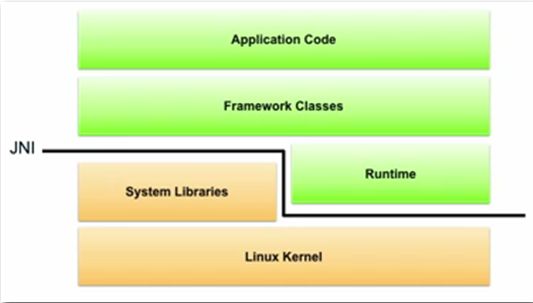
\includegraphics[width=.9\linewidth]{./pic/androidFramework.png}
\item 使用JNI时的Android框架 : 
\begin{itemize}
\item 绕过Framework提供的调用底层的代码, 直接调用自己写的C代码, 该代码最终会编译成为一个库, 这个库通过JNI提供的一个Stable的ABI 调用linux kernel;ABI是二进制程序接口 application binary interface.
\end{itemize}
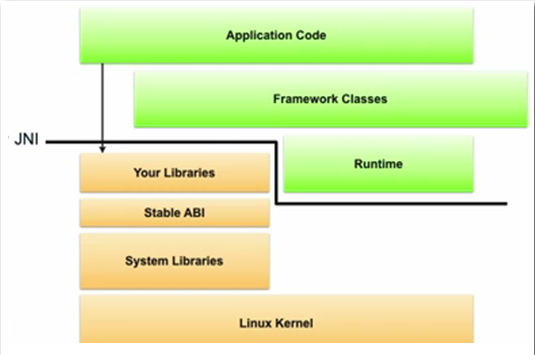
\includegraphics[width=.9\linewidth]{./pic/androidFrameworkJNI.png}
\end{itemize}
\subsection{JNI作用}
\label{sec-1-3}
\subsubsection{JNI作用 :}
\label{sec-1-3-1}
\begin{itemize}
\item \textbf{扩展}: JNI扩展了JVM能力, 驱动开发, 例如开发一个wifi驱动, 可以将手机设置为无限路由;
\item \textbf{高效} : 本地代码效率高, 游戏渲染, 音频视频处理等方面使用JNI调用本地代码, C语言可以灵活操作内存;
\item \textbf{复用} : 在文件压缩算法 7zip开源代码库, 机器视觉 openCV开放算法库 等方面可以复用C平台上的代码, 不必在开发一套完整的Java体系, 避免重复发明轮子;
\item \textbf{特殊} : 产品的核心技术一般也采用JNI开发, 不易破解;
\end{itemize}
\subsubsection{Java语言执行流程 :}
\label{sec-1-3-2}
\begin{itemize}
\item \textbf{编译字节码} : Java编译器编译 .java源文件, 获得.class 字节码文件;
\item \textbf{装载类库} : 使用类装载器装载平台上的Java类库, 并进行字节码验证;
\item \textbf{Java虚拟机} : 将字节码加入到JVM中, Java解释器 和 即时编译器 同时处理字节码文件, 将处理后的结果放入运行时系统;
\item \textbf{调用JVM所在平台类库} : JVM处理字节码后, 转换成相应平台的操作, 调用本平台底层类库进行相关处理;

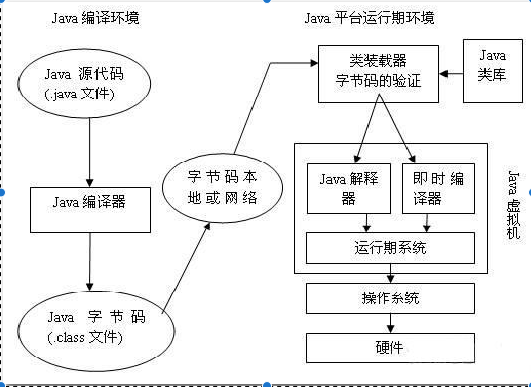
\includegraphics[width=.9\linewidth]{./pic/javaLanguage.png}

\item \textbf{Java一次编译到处执行} : JVM在不同的操作系统都有实现, Java可以一次编译到处运行, 字节码文件一旦编译好了, 可以放在任何平台的虚拟机上运行;
\end{itemize}
\subsection{NDK详解: 交叉编译库文件}
\label{sec-1-4}
\subsubsection{C代码执行 :}
\label{sec-1-4-1}
\begin{itemize}
\item C代码被编译成库文件之后, 才能执行, 库文件分为 动态库 和 静态库 两种;
\begin{itemize}
\item \textbf{动态库} : unix环境下 .so 后缀的是动态库, windows环境下 .dll 后缀的是动态库; 动态库可以依赖静态库加载一些可执行的C代码;
\item \textbf{静态库} : .a 后缀是静态库的扩展名;
\end{itemize}
\end{itemize}
\subsubsection{库文件来源 :}
\label{sec-1-4-2}
\begin{itemize}
\item C代码 进行 编译 链接操作之后, 才会生成库文件, 不同类型的CPU 操作系统 生成的库文件是不一样;
\begin{itemize}
\item \textbf{CPU分类} : arm结构, 嵌入式设备处理器; x86结构, pc 服务器处理器; 不同的CPU指令集不同;
\item \textbf{交叉编译} : windows x86编译出来的库文件可以在arm平台运行的代码;
\item \textbf{交叉编译工具链} : Google提供的 NDK 就是交叉编译工具链, 可以在linux环境下编译出在arn平台下执行的二进制库文件;
\end{itemize}
\item \textbf{NDK作用} : 
\begin{itemize}
\item 是Google提供了交叉编译工具链, 能够在 linux平台编译出在 arm平台下执行的二进制库文件;
\end{itemize}
\item \textbf{NDK版本介绍} : 
\begin{itemize}
\item android-ndk-windows 是在windows系统中的cygwin使用的, android-ndk-linux 是在linux下使用的;
\end{itemize}
\end{itemize}

\section{Android studio NDK ndk-build编译C生成 .so 文件步骤}
\label{sec-2}
\begin{itemize}
\item \url{https://blog.csdn.net/Mr_55/article/details/79773728}
\end{itemize}
\subsection{android.useDeprecatedDdk}
\label{sec-2-1}
\begin{itemize}
\item 新建一个demo项目jnidemo来记录JNI开发流程,项目创建完毕,打开gradle.properties文件,输入
\begin{minted}[linenos=true]{csharp}
android.useDeprecatedDdk=true
\end{minted}
\end{itemize}
,否者后面编译时会提示相关(so 库兼容错误)错误。

\subsection{配置NDK}
\label{sec-2-2}
\begin{itemize}
\item 配置gradle,打开app的gradle,在defaultConfig下面加入NDK的编译配置,这里的moduleName跟loadLibrary的时候用的名字必须相同:
\begin{minted}[linenos=true]{csharp}
  android {
      ndk {
          moduleName "myfirstndk" // 指定生成的so文件名
          abiFilters "x86", "x86_64", "arm64-v8a" // cpu的类型
      }
      sourceSets.main {
          jni.srcDirs = [] // 屏蔽掉默认的 jni 编译生成过程
          jniLibs.srcDir "src/main/libs"
      }
  }
  externalNativeBuild {
      ndkBuild {
          path "src/main/jni/Android.mk"
      }
  }
\end{minted}
\end{itemize}

\subsection{JniUtil.java}
\label{sec-2-3}
\begin{itemize}
\item 源文件
\begin{minted}[linenos=true]{java}
package com.myfirstndk;
public class JniUtil {
    static {
        // 加载生成 .so 文件名称
        System.loadLibrary("myfirstndk"); // 名字必须和build.gradle中的moduleName一致
    }
    public static native String sayHello(); // 底层映射
    // native 为本地的意思,顾名思义就是被表示为 sayHello() 函数是从本地映射上来的函数
}
\end{minted}
\item System.loadLibrary()方法加载动态库。(如果动态库的名字为libwgr.so,那么我们应该去掉文件名的lib和.so,只把中间的wgr作为参数传递到方法中进行加载)
\end{itemize}

\subsection{编译}
\label{sec-2-4}
\begin{itemize}
\item 用AS自带的命令行,进入到项目文件夹目录,输入命令 javac JniUtil.java,将java文件编译成.class文件:
\begin{minted}[linenos=true]{java}
javac JniUtil.java
\end{minted}
\end{itemize}

\subsection{生成头文件}
\label{sec-2-5}
\begin{itemize}
\item 输入命令
\begin{minted}[linenos=true]{csharp}
javah -jni com.myfirstndk.JniUtil // (包名+类名)
\end{minted}
\item 如果报找不到该类的错误,用
\begin{minted}[linenos=true]{csharp}
javah -classpath . -jni com.myfirstndk.JniUtil
\end{minted}
\item 此命令将生成与JniUtil类对应的.h文件。成功后将在包目录下生成一个 com\_myfirstndk\_JniUtil.h 文件。
\item javah -jni -d /自己想放入的目录(但是要方便自己寻找) -classpath . jni.JniPlug(切记JniPlug这个class文件在命令中是不要加.class后缀否则出错 )
\item 这样我们就有了需要的头文件了,不过我们要将这个头文件拷贝到我们项目中的一个制定文件夹,我的文件夹在src\main$\backslash$jni文件夹内为什么要建立这么一个文件夹呢?我们还需要配置Android.mk 与 Application.mk否则我们会在NDK-BUILD过程中报错。
\end{itemize}

\subsection{jni文件夹}
\label{sec-2-6}
\begin{itemize}
\item 新建一个jni文件夹,将刚刚生产的.h文件剪切到jni文件夹下面,并创建一个C/C++文件hello.c
\item hello.c的方法名必须跟.h文件中的方法名一致。这里的方法内容返回“HelloWorld!”
\begin{minted}[linenos=true]{c++}
#include "com_myfirstndk_JniUtil.h"
JNIEXPORT jstring JNICALL Java_com_myfirstndk_JniUtil_sayHello(JNIEnv *env, jclass jobj) {
    return (*env)->NewStringUTF(env, "Hello World~!");
}
\end{minted}
\end{itemize}

\subsection{建立android.mk}
\label{sec-2-7}
\begin{minted}[linenos=true]{csharp}
LOCAL_PATH := $(call my-dir)  # 为调用当前目录

include $(CLEAR_VARS)         # 清空无用变量

LOCAL_MODULE    := myfirstndk # 指定的是: 生成的库文件的名字(动态? 静态?)
LOCAL_SRC_FILES := hello.c    # 关联的是 jni 目录下的.c文件

# for logging
LOCAL_LDLIBS    += -llog

include $(BUILD_SHARED_LIBRARY) # 构建后成为共享库
\end{minted}

\subsection{建立Application.mk}
\label{sec-2-8}
\begin{minted}[linenos=true]{csharp}
APP_ABI := all  # ABI全部构建
\end{minted}

\subsection{通过ndk-build来生产库文件}
\label{sec-2-9}
\begin{itemize}
\item 通过alt+F12进入我们存放.h 与 Android.mk Application.mk文件的目录后,执行下面的命令
\item 命令行执行: 
\begin{minted}[linenos=true]{shell}
ndk-build NDK_PROJECT_PATH=. NDK_APPLICATION_MK=Application.mk APP_BUILD_SCRIPT=Android.mk
\end{minted}
\begin{itemize}
\item 解析
\begin{itemize}
\item ndk-build 为ndk命令方法, 默认的不用管
\item NDK\_PROJECT\_PATH=. 这是当前目录了,因为我们切换进来了在这里生产共享库文件
\item NDK\_APPLICATION\_MK=Application.mk 我们之前建立的文件
\item APP\_BUILD\_SCRIPT=Android.mk 我们之前建立的文件
\end{itemize}
\end{itemize}
\item 然后我们需要将生产的好库的上级目录一起拷贝到build.gradle文件中关键字 sourceSets.main设置的目录中就大功告成了
\end{itemize}

\subsection{Java配置项目}
\label{sec-2-10}
\begin{minted}[linenos=true]{java}
package com.myfirstndk;

import android.widget.TextView;
import android.os.Bundle;
import android.support.v7.app.AppCompatActivity;

public class MainActivity extends AppCompatActivity {
    @Override
    protected void onCreate(Bundle savedInstanceState) {
        super.onCreate(savedInstanceState);

        TextView tv = new TextView(this);
        tv.setText("the following came from jni: " + JniUtil.sayHello());
    }
}
\end{minted}


\section{Android NDK开发(1)----- Java与C互相调用}
\label{sec-3}
\begin{itemize}
\item \url{https://abc20899.iteye.com/blog/1861121}
\item callback.c文件如下:
\begin{minted}[linenos=true]{c}
#include <string.h>  
#include <stdio.h>  
#include <stdlib.h>  
#include <unistd.h>  
#include <sys/ioctl.h>  
#include <sys/types.h>  
#include <sys/stat.h>  
#include <fcntl.h>  
   
#include <jni.h>  
#include <android/log.h>  
   
#define LOGI(...) ((void)__android_log_print(
ANDROID_LOG_INFO, "native-activity", __VA_ARGS__))  
#define LOGW(...) ((void)__android_log_print(
ANDROID_LOG_WARN, "native-activity", __VA_ARGS__))  
   
/**********传输整数************* */  
JNIEXPORT void JNICALL Java_com_nan_callback_MyCallbackActivity_callJNIInt(
    JNIEnv* env, jobject obj , jint i) {  
    // 找到java中的类  
    jclass cls = (*env)->FindClass(env, "com/nan/callback/MyCallbackActivity");  
    // 再找类中的方法  
    jmethodID mid = (*env)->GetMethodID(env, cls, "callbackInt", "(I)V");  
    if (mid == NULL)    {  
        LOGI("int error");  
        return;    
    }  
    // 打印接收到的数据  
    LOGI("from java int: %d",i);  
    // 回调java中的方法  
    (*env)->CallVoidMethod(env, obj, mid ,i);  
           
}      
   
/********传输字符串**************/  
JNIEXPORT void JNICALL Java_com_nan_callback_MyCallbackActivity_callJNIString(
    JNIEnv* env, jobject obj , jstring s)   {  
    // 找到java中的类  
    jclass cls = (*env)->FindClass(env, "com/nan/callback/MyCallbackActivity");  
    // 再找类中的方法  
    jmethodID mid = (*env)->GetMethodID(
        env, cls, "callbackString", "(Ljava/lang/String;)V");  
    if (mid == NULL)    {  
        LOGI("string error");  
        return;    
    }  
    const char *ch;  
    // 获取由java传过来的字符串  
    ch = (*env)->GetStringUTFChars(env, s, NULL);  
    // 打印  
    LOGI("from java string: %s",ch);  
    (*env)->ReleaseStringUTFChars(env, s, ch);      
    // 回调java中的方法  
    (*env)->CallVoidMethod(env, obj, mid ,(*env)->NewStringUTF(env,"你好haha"));  
   
}  
   
/********传输数组(byte[])**************/  
JNIEXPORT void JNICALL Java_com_nan_callback_MyCallbackActivity_callJNIByte(
    JNIEnv* env, jobject obj , jbyteArray b)   {  
    // 找到java中的类  
    jclass cls = (*env)->FindClass(env, "com/nan/callback/MyCallbackActivity");  
    // 再找类中的方法  
    jmethodID mid = (*env)->GetMethodID(env, cls, "callbackByte", "([B)V");  
    if (mid == NULL)    {  
        LOGI("byte[] error");  
        return;    
    }  
       
    // 获取数组长度  
    jsize length = (*env)->GetArrayLength(env,b);  
    LOGI("length: %d",length);      
    // 获取接收到的数据  
    int i;  
    jbyte* p = (*env)->GetByteArrayElements(env,b,NULL);  
    // 打印  
    for(i=0;i<length;i++)   {  
        LOGI("%d",p[i]);      
    }  
   
    char c[5];  
    c[0] = 1;c[1] = 2;c[2] = 3;c[3] = 4;c[4] = 5;  
    // 构造数组  
    jbyteArray carr = (*env)->NewByteArray(env,length);  
    (*env)->SetByteArrayRegion(env,carr,0,length,c);  
    // 回调java中的方法  
    (*env)->CallVoidMethod(env, obj, mid ,carr);  
}
\end{minted}
\end{itemize}
% Emacs 25.3.1 (Org mode 8.2.7c)
\end{document}